%--------------------------------------------------------------------
%--------------------------------------------------------------------
% Formato para los talleres del curso de Métodos Computacionales
% Universidad de los Andes
% 2015, curso de vacaciones
%--------------------------------------------------------------------
%--------------------------------------------------------------------

\documentclass[11pt,letterpaper]{exam}
\usepackage[utf8]{inputenc}
\usepackage[spanish]{babel}
\usepackage{graphicx}
\usepackage{mdframed}
\usepackage{tabularx}
\usepackage[absolute]{textpos} % Para poner una imagen en posiciones arbitrarias
\usepackage{multirow}
\mdfdefinestyle{mystyle}{leftmargin=1cm,rightmargin=1cm,linecolor=red}
\usepackage{float}
\usepackage{hyperref}
\decimalpoint

\newcommand{\base}[1]{\underline{\hspace{#1}}}
\boxedpoints
\pointname{ pt}
%\extrawidth{0.75in}
%\extrafootheight{-0.5in}
\extraheadheight{-0.15in}
\hypersetup{%
  colorlinks=true,% hyperlinks will be coloured
  urlcolor=blue
}

%\noprintanswers
%\printanswers
\renewcommand{\solutiontitle}{}
\SolutionEmphasis{\color{blue}}

\usepackage{upquote,textcomp}
\newcommand\upquote[1]{\textquotesingle#1\textquotesingle} % To fix straight quotes in verbatim

\begin{document}
\begin{center}
{\Large Métodos Computacionales} \\
Tarea 3 - \textsc{Python}: \verb+matplotlib+ \\
Junio de 2015
\end{center}

\begin{textblock*}{40mm}(10mm,20mm)
  
\includegraphics[width=3cm]{logoUniandes.png}
\end{textblock*}

\begin{textblock*}{40mm}(164mm,20mm)
  
\includegraphics[width=3cm]{logoUniandes.png}
\end{textblock*}

\vspace{0.5cm}

La solución a esta tarea debe cargarse a su repositorio en GitHub en la carpeta /MC/Tareas/HW3/ y debe contener los archivos \verb+snowflake.ipynb+, \verb+Rayleigh.ipynb+, \verb+numsin.ipynb+. Es requisito que en todo lo hecho se pongan comentarios que expliquen lo que se está haciendo. La fecha límite para hacer un commit es el \textbf{jueves 18 de junio a las 23:59}. Puede trabajarse en parejas.

%\begin{textblock*}{100mm}(-430mm,130mm)
%  
\includegraphics[width=80cm]{koch6_tight.pdf}
%\end{textblock*}

\begin{textblock*}{100mm}(-4mm,-187mm)
  
\includegraphics[width=21cm]{koch6_tight.pdf}
\end{textblock*}

\vspace{0.5cm}

\begin{questions}
 
\question[40] \textbf{Koch Snowflake} \\
Programe en Python (20 pt) los seis primeros pasos de la construcción del \href{http://mathworld.wolfram.com/KochSnowflake.html}{Koch snowflake} y con ellos haga una animación como \href{https://github.com/ComputoCienciasUniandes/MetodosComputacionales/blob/master/homework/2015-V/HW3/snowflake.mp4?raw=true}{esta} (10 pt) y un panel (10 pt) como el que se muestra abajo. Guarde todo su trabajo en un notebook con nombre \verb+snowflake.ipynb+.

\vfill
\begin{center}
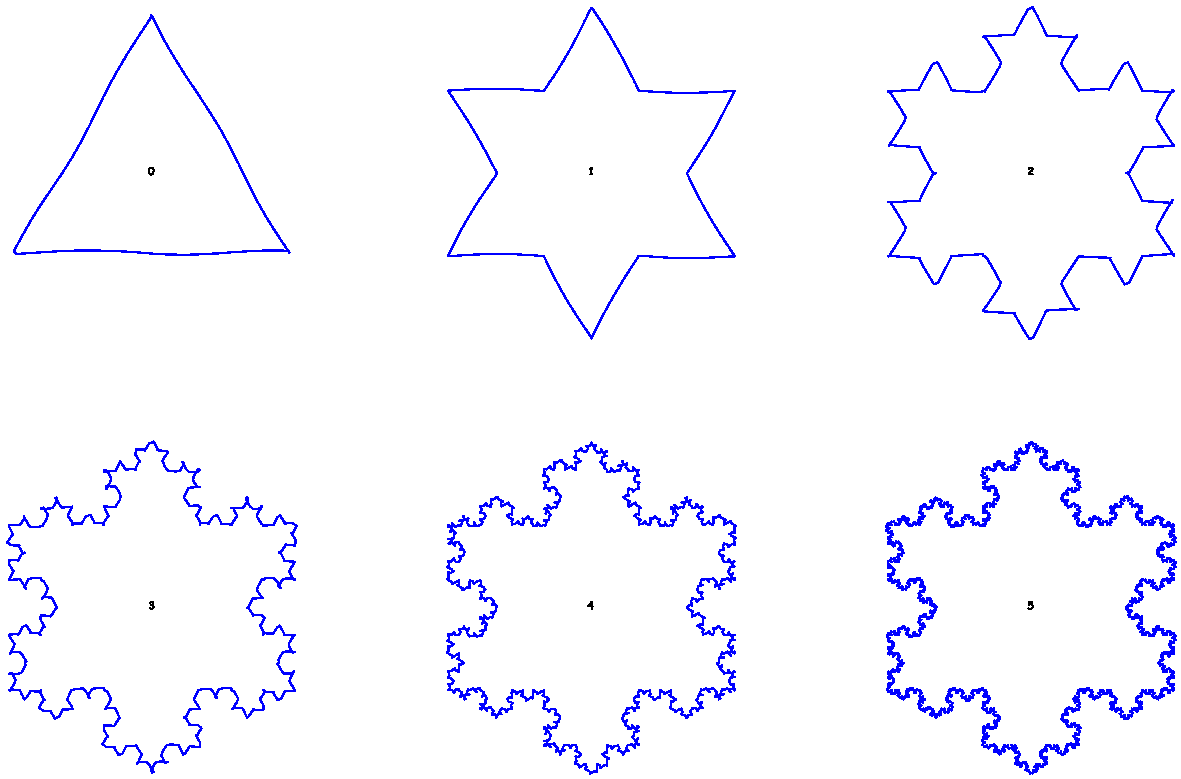
\includegraphics[width=0.9\textwidth]{kochpanel_tight.pdf}
\end{center}
\vfill
\newpage

\question[30] \textbf{Dinámica Molecular} \\

Lleve a cabo el experimento \href{https://github.com/ComputoCienciasUniandes/MetodosComputacionalesLaboratorio/blob/master/2015-V/actividades/experimentos/Exp1/Exp1.md}{aquí} descrito y haga un informe con las siguientes partes: introducción (10 pt), análisis de datos (10 pt) y conclusiones (10 pt). Tiene plena libertad para cambiar los parámetros del archivo de configuración \verb+pr_02_1.in+. La animación producida puede ser una película o un gif. Ambas la animación y la figura deben quedar renderizadas en la carpeta \verb+/MC/Tareas/HW3/+.

\vfill
\begin{center}
	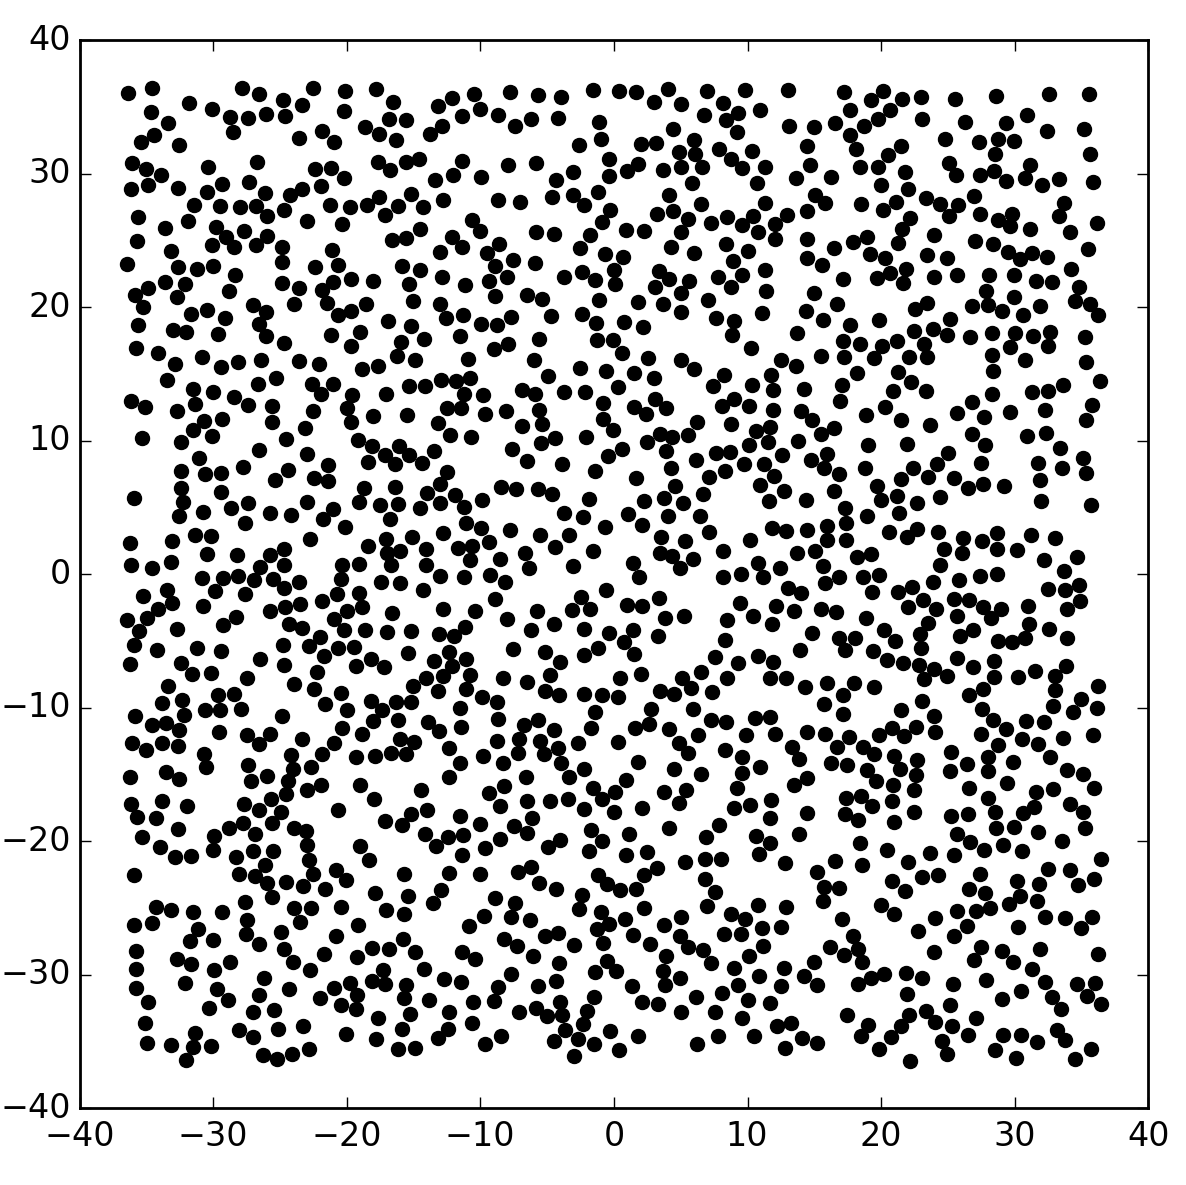
\includegraphics[width=0.95\textwidth]{./moldyn.png}
\end{center}
\vfill
\newpage

\question[30] \textbf{Error e incertidumbre en cálculos numéricos} \\

Lea los capítulos 1 y 2 del libro del {\it survey} de {\it Landau}.\\
Todo lo siguiente hágalo en un notebook de nombre \verb+numsin.ipynb+.\\[0.2cm]

\begin{parts}
	\part[10] Defina una función de Python llamada \verb+numsin+ que reciba dos cantidades, el número de términos a sumar en la serie de McLaurin para \verb+sin(x)+ y el valor de \verb+x+, y regrese la suma resultante. No utilice la función factorial, implemente el método explicado en la sección 1.8 del libro de {\it Landau}.
	
\[
	\sin(x) = \sum_{n=1}^{\infty}{ \left(-1\right)^{n-1}\frac{x^{2n-1}}{\left(2n-1\right)!} }	
\]

\begin{center}
	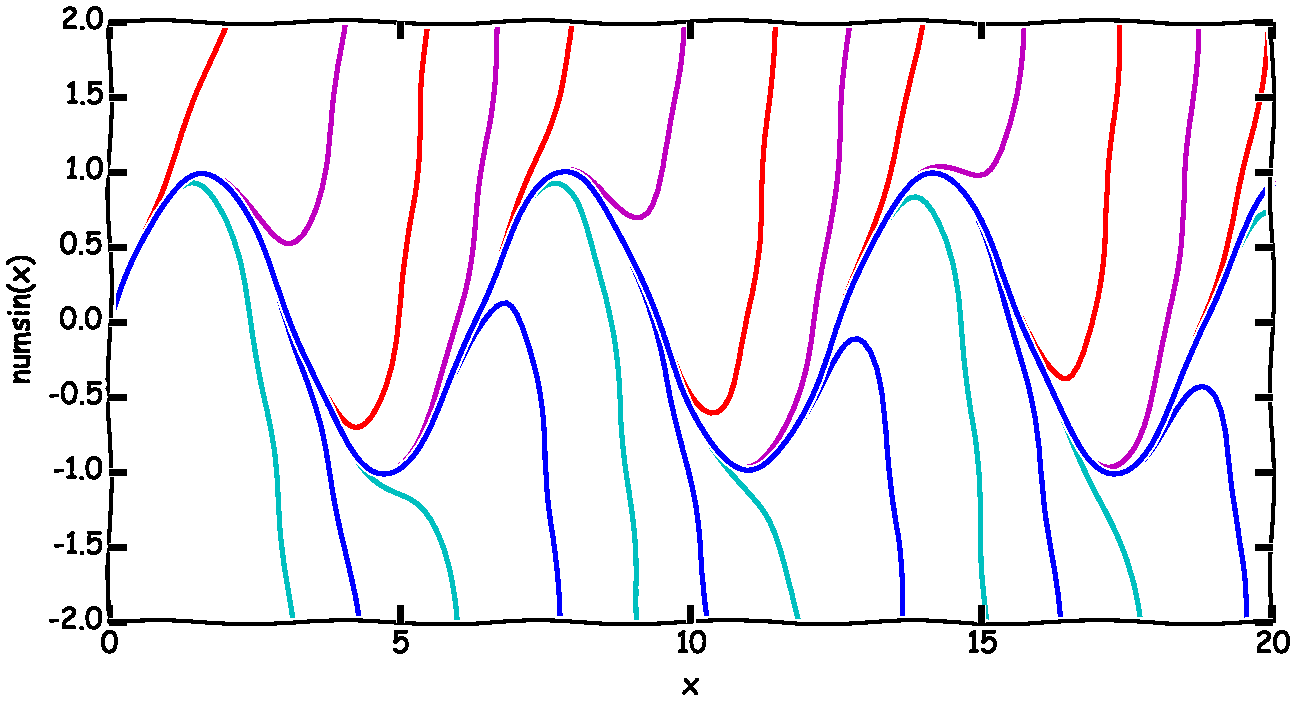
\includegraphics[width=0.9\textwidth]{./numsinxk.pdf}
\end{center}

	\part[20] Ahora calcule para cada elemento de \verb+linspace(0.,45,100)+ el número de términos a usar en \verb+numsin+ para que la magnitud de la diferencia entre el valor calculado con \verb+numsin+ y el ``real'' (usando la función \verb+sin+ de \verb+NumPy+) sea menor a \verb+0.01+. Al hacerlo va a encontrar dificultades, resuélvalas o explique la razón por la cual no pueden evitarse. Haga una gráfica que ayude a entender sus resultados.
\end{parts}




\end{questions}



\end{document}
